\documentclass[12pt,a4paper]{article}

\usepackage[utf8]{inputenc}
\usepackage[T1]{fontenc}
\usepackage[english]{babel}
\usepackage{geometry}
\geometry{margin=2.5cm}
\usepackage{graphicx}
\graphicspath{{img/}}
\usepackage{float}
\usepackage{listings}
\usepackage{xcolor}
\usepackage{hyperref}
\usepackage{fancyhdr}
\usepackage{booktabs}
\usepackage{array}
\usepackage{enumitem}
\usepackage{caption}

\hypersetup{colorlinks=true,linkcolor=black,urlcolor=blue,citecolor=black}

% ── Cisco IOS listings ──────────────────────────────────────────────────────
\definecolor{cmdbg}{RGB}{246,246,246}
\definecolor{cmdframe}{RGB}{185,185,185}
\definecolor{keyword}{RGB}{0,90,170}

\lstdefinestyle{cisco}{
  backgroundcolor=\color{cmdbg},
  frame=single,
  rulecolor=\color{cmdframe},
  basicstyle=\ttfamily\small,
  breaklines=true,
  columns=fullflexible,
  keepspaces=true,
  showstringspaces=false,
  xleftmargin=6pt, xrightmargin=6pt,
  aboveskip=8pt, belowskip=8pt,
  morekeywords={enable,configure,terminal,hostname,vlan,name,exit,end,
    interface,range,switchport,mode,access,trunk,allowed,no,shutdown,ip,address,
    default-gateway,dhcp,pool,network,default-router,dns-server,excluded-address,
    show,running-config,startup-config,copy,brief,spanning-tree,root,primary,
    secondary,fastEthernet,gigabitEthernet,cdp,run,neighbors,description,ping,
    route,encapsulation,dot1Q,router,ospf,area,passive-interface,router-id},
  keywordstyle=\color{keyword}\bfseries,
}
\lstset{style=cisco}


\pagestyle{fancy}
\fancyhf{}
\fancyhead[L]{\small Three-Building Campus Network}
\fancyhead[R]{\small\thepage}
\renewcommand{\headrulewidth}{0.4pt}

\title{%
  \vspace{-1cm}
  \textbf{Design and Configuration of a\\Three-Building Campus Network}\\[8pt]
  \large Technical Report}
\author{Mureșan Davide-Andrei\\[4pt]
Supervisor: Prof. Dr. Eng. Adrian Peculea\\
Technical University of Cluj-Napoca}
\date{2026}

\begin{document}
\maketitle
\thispagestyle{fancy}
\tableofcontents
\newpage

% ═════════════════════════════════════════════════════════════════════════════
\section{Overview}

\subsection{Scope}

A commercial institution occupies three buildings. Each building holds its own
user population and must stay reachable if a single inter-building link fails.
Four public services --- web, file transfer, name resolution and mail --- are
published from a demilitarised zone, and a link to an Internet provider is
established.

Three address blocks are given: \texttt{172.16.0.0/16} for the intranet,
\texttt{210.1.1.64/27} for the DMZ, and \texttt{210.1.1.32/27} for the provider
link.

\subsection{What was built}

\begin{table}[H]
\centering
\begin{tabular}{@{} l p{9.5cm} @{}}
\toprule
\textbf{Area} & \textbf{Implementation} \\
\midrule
Segmentation & Two VLANs per building --- one for users, one for management ---
  carried between switches over 802.1Q trunks. \\
Redundancy & Three switches per building cabled in a triangle, resolved by
  Spanning Tree; three routers in a full mesh, resolved by OSPF. \\
Addressing & DHCP served by each building router; infrastructure addresses
  static and excluded from the pools. \\
Access media & Cabled hosts and WPA2-protected wireless clients share the same
  user VLAN. \\
Routing & OSPF area 0 between the three building routers, with equal-cost
  multipath over the mesh. \\
Public services & HTTP, FTP, DNS and mail on public addresses in a dedicated
  DMZ, reachable both internally and from outside. \\
External link & Point-to-point connection to a provider router, with a simulated
  external network behind it. \\
Automation & Eight of the twelve device configurations generated from a single
  YAML inventory through Jinja2 templates. \\
\bottomrule
\end{tabular}
\end{table}

\subsection{Design decisions}

\begin{table}[H]
\centering
\renewcommand{\arraystretch}{1.25}
\begin{tabular}{@{} l p{9cm} @{}}
\toprule
\textbf{Decision} & \textbf{Reason} \\
\midrule
Separate management VLAN &
  A compromised user host does not share a broadcast domain with the switch
  management plane. \\
802.1Q trunking &
  Without it, a VLAN cannot traverse a switch, and segmentation would be
  indistinguishable from separate physical networks. \\
\texttt{/30} on point-to-point links &
  A link with two endpoints needs two usable addresses. A \texttt{/24} would
  waste 252 per link. \\
Explicit spanning-tree root &
  Otherwise the Layer~2 topology is decided by MAC addresses, that is, by
  chance. \\
Dedicated DMZ switch &
  The DMZ is a separate Layer~2 domain with its own VLAN and managed interface,
  not servers attached to an internal switch. \\
Static addresses for servers &
  A service that changes address is a service nobody can find. \\
Configuration generated from an inventory &
  The addressing plan and the running configuration cannot drift apart. \\
\bottomrule
\end{tabular}
\end{table}

\newpage
\subsection{Topology}

\begin{figure}[H]
\centering
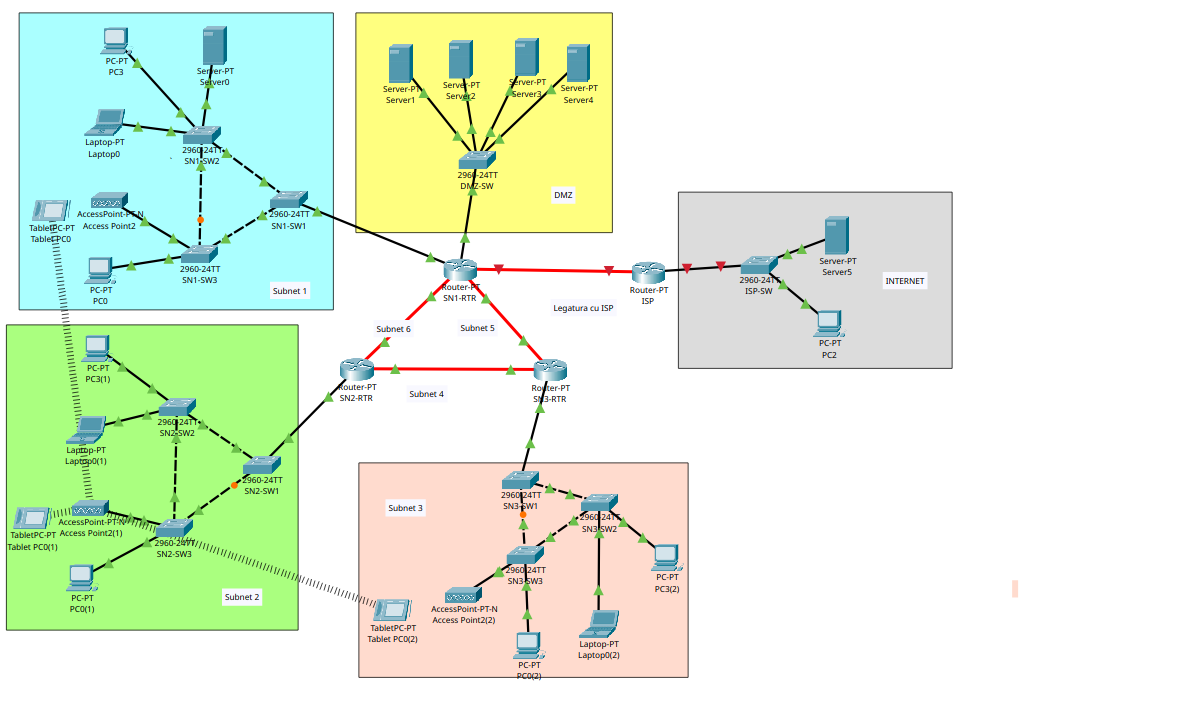
\includegraphics[width=1.4\textwidth]{topologie-generala.png}
\caption{Network topology in Cisco Packet Tracer. Three user zones, a DMZ, and a
  simulated external network.}
\end{figure}

\begin{table}[H]
\centering
\caption{Logical organisation}
\begin{tabular}{@{} l l l c c @{}}
\toprule
\textbf{Zone} & \textbf{Router} & \textbf{Switches} & \textbf{User VLAN} & \textbf{Mgmt VLAN} \\
\midrule
Subnet 1 & \texttt{SN1-RTR} & \texttt{SN1-SW1/2/3} & 10 & 110 \\
Subnet 2 & \texttt{SN2-RTR} & \texttt{SN2-SW1/2/3} & 20 & 120 \\
Subnet 3 & \texttt{SN3-RTR} & \texttt{SN3-SW1/2/3} & 30 & 130 \\
DMZ      & on \texttt{SN1-RTR} & \texttt{DMZ-SW}   & 200 & --- \\
External & \texttt{ISP}     & \texttt{ISP-SW}      & --- & --- \\
\bottomrule
\end{tabular}
\end{table}

\texttt{SN1-RTR} serves zone Subnet~1 and additionally holds the DMZ and the
provider uplink.

\subsection{Equipment}

Four routers (Router-PT), eleven switches (Cisco 2960-24TT), three access points
(AccessPoint-PT-N), six servers, and desktop, laptop and tablet clients.


% ═════════════════════════════════════════════════════════════════════════════
\newpage
\section{Addressing Plan}

\subsection{Sizing}

The number of usable hosts in a subnet with prefix $p$ is $2^{(32-p)} - 2$. Two
addresses are always unavailable: the network address, where all host bits are
zero, and the broadcast address, where all host bits are one.

The specification requires at least 200 users per subnet:

\begin{center}
\begin{tabular}{@{} c c c l @{}}
\toprule
\textbf{Host bits} & \textbf{Prefix} & \textbf{Usable} & \\
\midrule
7 & \texttt{/25} & 126 & insufficient \\
8 & \texttt{/24} & 254 & smallest prefix that satisfies the requirement \\
\bottomrule
\end{tabular}
\end{center}

\subsection{Intranet}

The \texttt{/16} block yields 256 subnets of size \texttt{/24} when eight bits
are borrowed for the network portion. The third octet becomes the subnet number.

\begin{table}[H]
\centering
\begin{tabular}{@{} c l l l @{}}
\toprule
\textbf{VLAN} & \textbf{Subnet} & \textbf{Purpose} & \textbf{Gateway} \\
\midrule
10  & \texttt{172.16.10.0/24}  & Subnet 1 users      & \texttt{172.16.10.1} \\
20  & \texttt{172.16.20.0/24}  & Subnet 2 users      & \texttt{172.16.20.1} \\
30  & \texttt{172.16.30.0/24}  & Subnet 3 users      & \texttt{172.16.30.1} \\
110 & \texttt{172.16.110.0/24} & Subnet 1 management & \texttt{172.16.110.1} \\
120 & \texttt{172.16.120.0/24} & Subnet 2 management & \texttt{172.16.120.1} \\
130 & \texttt{172.16.130.0/24} & Subnet 3 management & \texttt{172.16.130.1} \\
--- & \texttt{172.16.255.0/24} & Point-to-point links & --- \\
\bottomrule
\end{tabular}
\end{table}

Two conventions apply. The VLAN identifier equals the third octet, so
\texttt{172.16.20.55} identifies zone Subnet~2 without a lookup table.
Infrastructure links occupy the last \texttt{/24}, leaving user subnets free to
grow upward from \texttt{172.16.0.0}.

Within each user subnet, \texttt{.1--.9} are reserved for network equipment and
excluded from DHCP; \texttt{.10--.254} are allocated dynamically.

\subsection{Point-to-point links}

A router-to-router link has exactly two endpoints, so \texttt{/30} is an exact
fit: $2^2 - 2 = 2$ usable addresses. The block \texttt{172.16.255.0/24} divides
into 64 such subnets, stepping by four.

\begin{table}[H]
\centering
\begin{tabular}{@{} l c c c c @{}}
\toprule
\textbf{Block} & \textbf{Network} & \textbf{Host A} & \textbf{Host B} & \textbf{Broadcast} \\
\midrule
\texttt{172.16.255.0/30} & \texttt{.0} & \texttt{.1} & \texttt{.2}  & \texttt{.3}  \\
\texttt{172.16.255.4/30} & \texttt{.4} & \texttt{.5} & \texttt{.6}  & \texttt{.7}  \\
\texttt{172.16.255.8/30} & \texttt{.8} & \texttt{.9} & \texttt{.10} & \texttt{.11} \\
\bottomrule
\end{tabular}
\end{table}

The mask follows from the prefix: thirty network bits set to one and two host
bits set to zero give \texttt{255.255.255.252}, since
$128+64+32+16+8+4 = 252$.

\subsection{Public blocks}

Both \texttt{/27} blocks arrive already subnetted and their key addresses fixed.

\begin{table}[H]
\centering
\caption{\texttt{210.1.1.32/27} --- provider link}
\begin{tabular}{@{} l l @{}}
\toprule
\texttt{210.1.1.32}        & network address \\
\texttt{210.1.1.33}        & ISP router \\
\texttt{210.1.1.34}        & \texttt{SN1-RTR}, WAN interface \\
\texttt{210.1.1.35 -- .62} & reserved for address translation \\
\texttt{210.1.1.63}        & broadcast address \\
\bottomrule
\end{tabular}
\end{table}

\begin{table}[H]
\centering
\caption{\texttt{210.1.1.64/27} --- DMZ}
\begin{tabular}{@{} l l l @{}}
\toprule
\textbf{Address} & \textbf{Device} & \textbf{Name} \\
\midrule
\texttt{210.1.1.65} & \texttt{SN1-RTR}, DMZ interface & --- \\
\texttt{210.1.1.66} & HTTP server & \texttt{www.davide.ro} \\
\texttt{210.1.1.67} & FTP server  & \texttt{ftp.davide.ro} \\
\texttt{210.1.1.68} & DNS server  & \texttt{dns.davide.ro} \\
\texttt{210.1.1.69} & Mail server & \texttt{mail.davide.ro} \\
\texttt{210.1.1.70} & \texttt{DMZ-SW}, management interface & --- \\
\bottomrule
\end{tabular}
\end{table}

\newpage
% ═════════════════════════════════════════════════════════════════════════════
\part*{Part I --- Foundation}
\addcontentsline{toc}{part}{Part I --- Foundation}

% ═════════════════════════════════════════════════════════════════════════════
\section{Naming and Topology Discovery}

Devices arrived with factory default names: every router was \texttt{Router} and
every switch \texttt{Switch}. The labels shown on the Packet Tracer workspace are
independent of the configured hostname and do not appear in network protocols, so
neighbour discovery was unusable:

\begin{lstlisting}
Device ID    Local Intrfce   Holdtme   Capability   Platform   Port ID
Switch       Fas 1/0          138          S        2960       Fas 0/1
Switch       Fas 0/0          138          S        2960       Fas 0/4
\end{lstlisting}

Two different switches, one in Subnet~1 and one in the DMZ, reporting the same
identifier.

\subsection{Naming convention}

Names follow the zones already present in the topology, so no translation is
needed between the diagram and the command line.

\begin{table}[H]
\centering
\begin{tabular}{@{} l l @{}}
\toprule
\texttt{SNx-RTR} & zone router \\
\texttt{SNx-SW1} & switch connected to the router; spanning-tree root \\
\texttt{SNx-SW2}, \texttt{SNx-SW3} & access switches \\
\texttt{DMZ-SW}, \texttt{ISP}, \texttt{ISP-SW} & DMZ and external network \\
\bottomrule
\end{tabular}
\end{table}

\subsection{Configuration}

On each of the fifteen devices:

\begin{lstlisting}
enable
configure terminal
hostname SN2-RTR
end
\end{lstlisting}

Routers additionally required CDP to be enabled and their interfaces brought up.
Unlike switch ports, router interfaces are administratively shut down from the
factory:

\begin{lstlisting}
configure terminal
cdp run
interface gigabitEthernet 6/0
 no shutdown
interface gigabitEthernet 7/0
 no shutdown
end
\end{lstlisting}

\subsection{Discovery}

With unique names in place, CDP became readable:

\begin{lstlisting}
SN3-RTR#show cdp neighbors
Device ID    Local Intrfce   Holdtme   Capability   Platform   Port ID
SN2-RTR      Gig 6/0          145          R        PT1000     Gig 6/0
SN1-RTR      Gig 7/0          145          R        PT1000     Gig 7/0
SN3-SW1      Fas 0/0          145          S        2960       Fas 0/1
\end{lstlisting}

Queries from all four routers and all nine switches agree with one another, each
link appearing from both ends with matching ports.

\begin{table}[H]
\centering
\caption{Port map}
\begin{tabular}{@{} l l l l l @{}}
\toprule
\textbf{Device} & \textbf{Interface} & \textbf{Neighbour} & \textbf{Remote} & \textbf{Purpose} \\
\midrule
\texttt{SN1-RTR} & \texttt{Fa0/0} & \texttt{SN1-SW1} & \texttt{Fa0/4} & LAN uplink \\
\texttt{SN1-RTR} & \texttt{Fa1/0} & \texttt{DMZ-SW}  & \texttt{Fa0/1} & DMZ \\
\texttt{SN1-RTR} & \texttt{Gi6/0} & \texttt{ISP}     & \texttt{Gi6/0} & WAN, fibre \\
\texttt{SN1-RTR} & \texttt{Gi7/0} & \texttt{SN3-RTR} & \texttt{Gi7/0} & transit \\
\texttt{SN1-RTR} & \texttt{Gi8/0} & \texttt{SN2-RTR} & \texttt{Gi7/0} & transit \\
\texttt{SN2-RTR} & \texttt{Fa0/0} & \texttt{SN2-SW1} & \texttt{Fa0/3} & LAN uplink \\
\texttt{SN2-RTR} & \texttt{Gi6/0} & \texttt{SN3-RTR} & \texttt{Gi6/0} & transit \\
\texttt{SN3-RTR} & \texttt{Fa0/0} & \texttt{SN3-SW1} & \texttt{Fa0/1} & LAN uplink \\
\texttt{ISP}     & \texttt{Fa0/0} & \texttt{ISP-SW}  & \texttt{Fa0/1} & external \\
\bottomrule
\end{tabular}
\end{table}

Router-to-router links run on GigabitEthernet, access uplinks on FastEthernet ---
a fast core with slower edges, as in any campus network.

% ═════════════════════════════════════════════════════════════════════════════
\section{Routing Backbone}

The three routers are cabled in a triangle. Any one link may fail without
partitioning the network.

\begin{figure}[H]
\centering
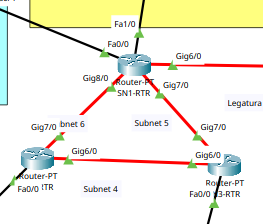
\includegraphics[width=0.6\textwidth]{triunghi-routere.png}
\caption{The three transit links between zone routers.}
\end{figure}

\begin{table}[H]
\centering
\begin{tabular}{@{} l l l @{}}
\toprule
\textbf{Subnet} & \textbf{Endpoint A} & \textbf{Endpoint B} \\
\midrule
\texttt{172.16.255.0/30} & \texttt{SN1-RTR Gi8/0} $\to$ \texttt{.1}
                         & \texttt{SN2-RTR Gi7/0} $\to$ \texttt{.2} \\
\texttt{172.16.255.4/30} & \texttt{SN2-RTR Gi6/0} $\to$ \texttt{.5}
                         & \texttt{SN3-RTR Gi6/0} $\to$ \texttt{.6} \\
\texttt{172.16.255.8/30} & \texttt{SN1-RTR Gi7/0} $\to$ \texttt{.9}
                         & \texttt{SN3-RTR Gi7/0} $\to$ \texttt{.10} \\
\bottomrule
\end{tabular}
\end{table}

Both endpoints of a link necessarily belong to the same \texttt{/30}; otherwise
the link carries traffic while the routers fail to recognise each other as
neighbours.

\begin{lstlisting}
SN1-RTR(config)#interface gigabitEthernet 8/0
SN1-RTR(config-if)# description Transit to SN2-RTR
SN1-RTR(config-if)# ip address 172.16.255.1 255.255.255.252
SN1-RTR(config-if)# no shutdown
\end{lstlisting}

The \texttt{description} has no functional effect but records the purpose of the
interface where it remains visible in \texttt{show running-config}.

\subsection{Verification}

\begin{lstlisting}
SN1-RTR#show ip interface brief
Interface              IP-Address      OK? Method Status  Protocol
GigabitEthernet7/0     172.16.255.9    YES manual up      up
GigabitEthernet8/0     172.16.255.1    YES manual up      up
\end{lstlisting}

All three sides of the triangle respond:

\begin{center}
\begin{tabular}{@{} l l c @{}}
\toprule
\textbf{Source} & \textbf{Destination} & \textbf{Success} \\
\midrule
\texttt{SN1-RTR} & \texttt{172.16.255.2}  & 100\% \\
\texttt{SN1-RTR} & \texttt{172.16.255.10} & 100\% \\
\texttt{SN2-RTR} & \texttt{172.16.255.6}  & 100\% \\
\bottomrule
\end{tabular}
\end{center}

The first run of each test returns 80\%: the initial packet is held while ARP
resolves the destination hardware address. Subsequent runs return 100\%.

\subsection{Limits at this point}

A ping from \texttt{SN2-RTR} to \texttt{172.16.255.10} fails:

\begin{lstlisting}
SN2-RTR#ping 172.16.255.10
.....
Success rate is 0 percent (0/5)
\end{lstlisting}

This is correct behaviour. The router knows only its directly connected networks:

\begin{lstlisting}
C    172.16.255.0/30 is directly connected, GigabitEthernet7/0
C    172.16.255.4/30 is directly connected, GigabitEthernet6/0
\end{lstlisting}

The address \texttt{172.16.255.10} belongs to the link between \texttt{SN1-RTR}
and \texttt{SN3-RTR}, which \texttt{SN2-RTR} is not attached to. Without a
routing protocol it has no way of learning that the network exists. This test is
repeated once OSPF is running.

% ═════════════════════════════════════════════════════════════════════════════
\newpage
\section{VLANs and Layer 2 Switching}

Each zone holds three switches cabled in a triangle --- a Layer~2 loop. Unlike IP
packets, Ethernet frames carry no time-to-live field, so a single broadcast
entering a loop circulates indefinitely, duplicating at every switch until the
zone saturates.

Spanning Tree elects a root bridge and blocks the port that closes the loop,
keeping it as a standby path.

\subsection{Port roles}

\begin{table}[H]
\centering
\begin{tabular}{@{} l p{9cm} @{}}
\toprule
\textbf{Access port} & Belongs to one VLAN. End devices connect here and remain
  unaware that VLANs exist. \\
\textbf{Trunk port} & Carries several VLANs over one cable, each frame tagged
  with its VLAN identifier per IEEE~802.1Q. \\
\textbf{SVI} & A virtual interface giving the switch an address inside a VLAN.
  Needed for remote administration, not for forwarding. \\
\bottomrule
\end{tabular}
\end{table}

\subsection{Per-zone values}

\begin{table}[H]
\centering
\begin{tabular}{@{} l c c l l l @{}}
\toprule
\textbf{Zone} & \textbf{Users} & \textbf{Mgmt} & \textbf{SW1} & \textbf{SW2} & \textbf{SW3} \\
\midrule
Subnet 1 & 10 & 110 & \texttt{172.16.110.2} & \texttt{.3} & \texttt{.4} \\
Subnet 2 & 20 & 120 & \texttt{172.16.120.2} & \texttt{.3} & \texttt{.4} \\
Subnet 3 & 30 & 130 & \texttt{172.16.130.2} & \texttt{.3} & \texttt{.4} \\
\bottomrule
\end{tabular}
\end{table}

\texttt{SW1} is \texttt{root primary} in every zone, \texttt{SW2} is
\texttt{root secondary}, \texttt{SW3} keeps the default priority.

\subsection{Configuration}

Shown for \texttt{SN2-SW1}, which carries three trunks.

\begin{lstlisting}
vlan 20
 name Users-SN2
exit
vlan 120
 name Mgmt-SN2
exit

interface fastEthernet 0/1
 description Trunk to SN2-SW2
 switchport mode trunk
 switchport trunk allowed vlan 20,120
exit

interface range fastEthernet 0/4-24
 switchport mode access
 switchport access vlan 20
exit

interface vlan 120
 ip address 172.16.120.2 255.255.255.0
 no shutdown
exit

ip default-gateway 172.16.120.1
spanning-tree vlan 20,120 root primary
\end{lstlisting}

Three details carry weight:

\begin{itemize}[nosep]
  \item A VLAN must exist on every switch its traffic crosses. Tagged frames for
        an unknown VLAN are discarded on arrival.
  \item \texttt{switchport trunk allowed vlan} restricts the link to the two
        VLANs in use. A trunk permits all 4094 by default, which both floods
        unnecessary traffic and opens a path for VLAN hopping.
  \item \texttt{switchport mode access} fixes the port role. Left unset, a port
        stays in dynamic mode and can be negotiated into a trunk by an attacking
        device.
\end{itemize}

Unused ports are configured as well. A port left in the default VLAN~1 is a port
through which an unauthorised device reaches the network immediately.

\subsection{Spanning-tree priorities}

\begin{table}[H]
\centering
\begin{tabular}{@{} l l c c @{}}
\toprule
\textbf{Switch} & \textbf{Command} & \textbf{Configured} & \textbf{Effective} \\
\midrule
\texttt{SN2-SW1} & \texttt{root primary}   & $32768-8192 = 24576$ & 24596 \\
\texttt{SN2-SW2} & \texttt{root secondary} & $32768-4096 = 28672$ & 28692 \\
\texttt{SN2-SW3} & ---                     & 32768                & 32788 \\
\bottomrule
\end{tabular}
\end{table}

The effective value adds the VLAN identifier, since a separate spanning-tree
instance runs per VLAN. \texttt{SW1} is chosen as root because it holds the
uplink to the router; placing the root elsewhere would make outbound traffic
cross the zone twice.

\subsection{Verification}

\begin{lstlisting}
SN2-SW1#show interface trunk
Port        Mode    Encapsulation  Status     Native vlan
Fa0/1       on      802.1q         trunking   1
Fa0/2       on      802.1q         trunking   1
Fa0/3       on      802.1q         trunking   1

Port        Vlans allowed on trunk
Fa0/1       20,120
\end{lstlisting}

\begin{lstlisting}
SN2-SW3#show spanning-tree vlan 20
  Root ID    Priority    24596
             Address     00D0.58B9.4CAC
             Cost        19
             Port        4(FastEthernet0/4)

  Bridge ID  Priority    32788  (priority 32768 sys-id-ext 20)

Interface        Role Sts Cost      Prio.Nbr Type
---------------- ---- --- --------- -------- ------------------------
Fa0/1            Desg FWD 19        128.1    Shr
Fa0/2            Altn BLK 19        128.2    P2p
Fa0/3            Desg FWD 19        128.3    P2p
Fa0/4            Root FWD 19        128.4    P2p
\end{lstlisting}

The root is \texttt{SN2-SW1}; \texttt{Fa0/4} is the root port, the lowest-cost
path towards it; \texttt{Fa0/2} is blocked. Exactly one port is blocked per zone,
which is the expected result for a topology containing one loop.

\subsection{Redundancy in effect}

All three switches hold addresses in the management VLAN, so reachability between
them exercises the whole Layer~2 configuration:

\begin{lstlisting}
SN2-SW3#ping 172.16.120.3
!!!!!
Success rate is 100 percent (5/5)
\end{lstlisting}

The result is more informative than it appears. \texttt{172.16.120.3} belongs to
\texttt{SN2-SW2}, and the port connecting \texttt{SN2-SW3} directly to it is
blocked. The traffic therefore travels around the triangle, through
\texttt{SN2-SW1}. The loop is eliminated while connectivity is preserved; should
the active link fail, the blocked port is unblocked and traffic resumes over the
standby path.

% ═════════════════════════════════════════════════════════════════════════════
\section{Inter-VLAN Routing}

The zone router has one physical interface towards the zone but needs two
addresses --- a gateway for each VLAN. The interface is divided into logical
sub-interfaces, one per VLAN. Frames arrive tagged over the trunk, and the router
delivers each to the matching sub-interface.

\begin{lstlisting}
interface fastEthernet 0/0
 no ip address
 no shutdown
exit

interface fastEthernet 0/0.20
 description Users VLAN 20
 encapsulation dot1Q 20
 ip address 172.16.20.1 255.255.255.0
exit

interface fastEthernet 0/0.120
 description Management VLAN 120
 encapsulation dot1Q 120
 ip address 172.16.120.1 255.255.255.0
exit
\end{lstlisting}

The physical interface carries no address. The number after the dot is a local
identifier, set equal to the VLAN for readability; the actual binding is made by
\texttt{encapsulation dot1Q}. Sub-interfaces inherit the state of the physical
interface and need no \texttt{no shutdown}.

\subsection{Verification}

\begin{lstlisting}
SN2-RTR#show ip interface brief
Interface              IP-Address      OK? Method Status  Protocol
FastEthernet0/0        unassigned      YES unset  up      up
FastEthernet0/0.20     172.16.20.1     YES manual up      up
FastEthernet0/0.120    172.16.120.1    YES manual up      up
\end{lstlisting}

A host in the user VLAN reaching a switch in the management VLAN:

\begin{lstlisting}
C:\>ping 172.16.120.3
Reply from 172.16.120.3: bytes=32 time=16ms TTL=254
Reply from 172.16.120.3: bytes=32 time<1ms TTL=254
Packets: Sent = 4, Received = 4, Lost = 0 (0% loss)
\end{lstlisting}

The two hosts sit in networks separated at Layer~2, so the traffic must traverse
the router. The TTL confirms it independently: each router decrements the field
by one, and the reply arrives with 254 instead of 255. A ping to the gateway
itself returns \texttt{TTL=255}, since no router is crossed.

\subsection{Fault isolation}

During verification, one test failed while its equivalents succeeded:

\begin{table}[H]
\centering
\begin{tabular}{@{} l l c @{}}
\toprule
\textbf{Source} & \textbf{Destination} & \textbf{Result} \\
\midrule
Host \texttt{172.16.20.50} & gateway \texttt{172.16.20.1}  & success \\
\texttt{SN2-RTR}           & switch \texttt{172.16.120.2}  & success \\
\texttt{SN2-SW2}           & host \texttt{172.16.20.50}    & success \\
Host \texttt{172.16.20.50} & switch \texttt{172.16.120.2}  & \textbf{failure} \\
\bottomrule
\end{tabular}
\end{table}

The asymmetry locates the cause. The router shares a subnet with the switches and
receives replies without the switch needing any routing knowledge. A host in a
different subnet does not: the switch receives the request, but to answer it must
forward the reply through its own default gateway. The switch in question was
missing \texttt{ip default-gateway}, so requests arrived and replies never left.

A failed ping does not distinguish between a request that never arrived and a
reply that never returned. Running the test from the opposite endpoint separates
the two cases.

% ═════════════════════════════════════════════════════════════════════════════
\newpage
\section{Dynamic Address Allocation}

Each zone router serves DHCP for its own user VLAN. This works because the router
is present inside the VLAN through its sub-interface and therefore receives the
broadcast discovery messages directly. A server placed in another VLAN would have
required \texttt{ip helper-address} on each sub-interface to convert those
broadcasts into directed unicasts.

\begin{lstlisting}
ip dhcp excluded-address 172.16.20.1 172.16.20.9

ip dhcp pool SN2-USERS
 network 172.16.20.0 255.255.255.0
 default-router 172.16.20.1
 dns-server 210.1.1.68
exit
\end{lstlisting}

\texttt{default-router} and \texttt{dns-server} do not configure the router; they
are values transmitted to clients. The exclusion is a global command and must
precede the pool --- without it, allocation would begin at the gateway's own
address.

The management VLAN is deliberately left out of DHCP. Infrastructure keeps static
addresses, so a switch cannot lose its management address to an expired lease.

\subsection{Verification}

\begin{lstlisting}
C:\>ipconfig /all
   Physical Address................: 0060.708B.8AE8
   IPv4 Address....................: 172.16.20.10
   Subnet Mask.....................: 255.255.255.0
   Default Gateway.................: 172.16.20.1
   DHCP Servers....................: 172.16.20.1
   DNS Servers.....................: 210.1.1.68
\end{lstlisting}

The allocated address is the first one after the excluded range, which
demonstrates that the exclusion took effect. The DHCP server is the router
itself, as required.

\begin{lstlisting}
SN2-RTR#show ip dhcp binding
IP address       Client-ID/              Lease expiration    Type
172.16.20.10     0060.708B.8AE8           --                 Automatic
\end{lstlisting}

The hardware address in the lease table matches the one reported by the client.

\subsection{A reporting quirk}

\texttt{show ip dhcp pool} reports \texttt{Excluded addresses: 1} although nine
addresses were excluded. Packet Tracer counts excluded \emph{ranges} rather than
individual addresses. The allocation beginning at \texttt{.10} is the
authoritative evidence.

% ═════════════════════════════════════════════════════════════════════════════
\newpage
\section{Wireless Access}

One access point per zone, connected to an access port in the user VLAN. Wireless
clients therefore land in the same VLAN as cabled hosts and draw addresses from
the same DHCP pool.

\begin{table}[H]
\centering
\begin{tabular}{@{} l l l l @{}}
\toprule
\textbf{Zone} & \textbf{SSID} & \textbf{Authentication} & \textbf{Encryption} \\
\midrule
Subnet 1 & \texttt{SN1-WiFi} & WPA2-PSK & AES \\
Subnet 2 & \texttt{SN2-WiFi} & WPA2-PSK & AES \\
Subnet 3 & \texttt{SN3-WiFi} & WPA2-PSK & AES \\
\bottomrule
\end{tabular}
\end{table}

Access points are configured through the device interface rather than a command
line. WPA2 with AES was selected over WPA with TKIP, which is deprecated.

\subsection{Verification}

A tablet associating and obtaining an address exercises the whole path at once:
the WPA2 handshake, the access point bridging into the VLAN, the DHCP request
reaching the router, and the reply returning.

\begin{lstlisting}
C:\>ipconfig /all
   IPv4 Address....................: 172.16.10.11
   Default Gateway.................: 172.16.10.1
   DNS Servers.....................: 210.1.1.68
\end{lstlisting}

The address follows the one held by the cabled host in the same zone, confirming
both media share a single pool. A ping from the tablet to that cabled host
succeeds, confirming they share one VLAN rather than forming parallel networks.

% ═════════════════════════════════════════════════════════════════════════════
\section{OSPF}

Without a routing protocol, each router knows only its directly connected
networks. Reaching the other zones would require static routes on every router
for every remote subnet --- fifteen entries in this topology --- and those routes
would not adapt when a link fails, defeating the purpose of the triangular
cabling.

OSPF is a link-state protocol: each router advertises its own links, all routers
build the same map, and each computes shortest paths independently using
Dijkstra's algorithm.

\subsection{Configuration}

\begin{lstlisting}
router ospf 1
 router-id 2.2.2.2
 network 172.16.20.0 0.0.0.255 area 0
 network 172.16.120.0 0.0.0.255 area 0
 network 172.16.255.0 0.0.0.3 area 0
 network 172.16.255.4 0.0.0.3 area 0
 passive-interface fastEthernet 0/0.20
 passive-interface fastEthernet 0/0.120
exit
\end{lstlisting}

\begin{table}[H]
\centering
\begin{tabular}{@{} l p{9cm} @{}}
\toprule
\texttt{router-id} & Set explicitly. Left unset, the router derives it from an
  interface address, so its identity changes if that interface does. \\
\texttt{network ... area 0} & Selects which interfaces participate. The wildcard
  mask is the inverse of the subnet mask: \texttt{0.0.0.255} for a \texttt{/24},
  \texttt{0.0.0.3} for a \texttt{/30}. \\
\texttt{passive-interface} & Suppresses Hello messages on user-facing
  sub-interfaces while still advertising their networks. No router lives there,
  and Hello packets on a user segment are both wasted traffic and free topology
  information for anyone listening. \\
\bottomrule
\end{tabular}
\end{table}

Transit links were additionally declared point-to-point:

\begin{lstlisting}
interface gigabitEthernet 6/0
 ip ospf network point-to-point
\end{lstlisting}

OSPF treats an Ethernet segment as broadcast by default and elects a designated
router. On a \texttt{/30} holding exactly two routers this election is
unnecessary and delays convergence.

\subsection{Verification}

\begin{lstlisting}
SN3-RTR#show ip ospf neighbor
Neighbor ID     Pri   State      Dead Time   Address         Interface
2.2.2.2           1   FULL       00:00:32    172.16.255.5    GigabitEthernet6/0
1.1.1.1           1   FULL       00:00:38    172.16.255.9    GigabitEthernet7/0
\end{lstlisting}

Two neighbours per router, both in \texttt{FULL} state --- the databases are
fully synchronised.

\begin{lstlisting}
SN2-RTR#show ip route

     172.16.0.0/16 is variably subnetted, 9 subnets, 2 masks
O       172.16.10.0/24 [110/2] via 172.16.255.1, GigabitEthernet7/0
C       172.16.20.0/24 is directly connected, FastEthernet0/0.20
O       172.16.30.0/24 [110/2] via 172.16.255.6, GigabitEthernet6/0
O       172.16.110.0/24 [110/2] via 172.16.255.1, GigabitEthernet7/0
C       172.16.120.0/24 is directly connected, FastEthernet0/0.120
O       172.16.130.0/24 [110/2] via 172.16.255.6, GigabitEthernet6/0
C       172.16.255.0/30 is directly connected, GigabitEthernet7/0
C       172.16.255.4/30 is directly connected, GigabitEthernet6/0
O       172.16.255.8/30 [110/2] via 172.16.255.1, GigabitEthernet7/0
                        [110/2] via 172.16.255.6, GigabitEthernet6/0
\end{lstlisting}

Routes marked \texttt{O} were learned through OSPF. The value \texttt{[110/2]}
gives the administrative distance, 110 for OSPF, and the path cost.

The entry for \texttt{172.16.255.8/30} lists \textbf{two next hops of equal
cost}. This is equal-cost multipath, a direct consequence of the triangular
topology: the network is reachable through either neighbour at the same cost, and
traffic is distributed across both.

The test that failed before OSPF was configured now succeeds, since
\texttt{SN2-RTR} has learned the network it previously had no knowledge of.

% ═════════════════════════════════════════════════════════════════════════════
\part*{Part II --- Services}
\addcontentsline{toc}{part}{Part II --- Services}

% ═════════════════════════════════════════════════════════════════════════════
\section{Demilitarised Zone}

The four public servers occupy a separate Layer~2 domain with its own switch and
VLAN, attached to \texttt{SN1-RTR} on a dedicated interface. Their addresses come
from \texttt{210.1.1.64/27} and are public, so no translation is involved in
reaching them.

VLAN~200 was chosen rather than 20, which is already in use as \texttt{Users-SN2}
in another zone. The two switches share no trunk, so the identifiers could
technically coexist, but reusing one across roles is a debugging trap.

\begin{lstlisting}
! on SN1-RTR
interface fastEthernet 1/0
 description DMZ
 ip address 210.1.1.65 255.255.255.224
 no shutdown
exit

router ospf 1
 network 210.1.1.64 0.0.0.31 area 0
 passive-interface fastEthernet 1/0
exit
\end{lstlisting}

\begin{lstlisting}
! on DMZ-SW
vlan 200
 name DMZ
exit

interface range fastEthernet 0/1-24
 switchport mode access
 switchport access vlan 200
exit

interface vlan 200
 ip address 210.1.1.70 255.255.255.224
 no shutdown
exit

ip default-gateway 210.1.1.65
\end{lstlisting}

No trunk is configured in the DMZ: a single VLAN has nothing to tag. No spanning
tree concerns arise either, since there is one switch and no loop.

Advertising \texttt{210.1.1.64/27} into OSPF is what allows the other two zones
to reach the servers. Without it, only \texttt{SN1-RTR} would know the network
exists. The interface is passive because the DMZ holds servers, not routers.

Servers hold static addresses, with \texttt{210.1.1.65} as gateway and
\texttt{210.1.1.68} as name server. The mask is \texttt{255.255.255.224};
accepting the default \texttt{/24} would make a server treat the entire
\texttt{210.1.1.0} range as local and never use its gateway.

\subsection{Verification}

From the DMZ gateway:

\begin{center}
\begin{tabular}{@{} l l c @{}}
\toprule
\textbf{Destination} & \textbf{Device} & \textbf{Success} \\
\midrule
\texttt{210.1.1.66} & HTTP server & 80\% then 100\% \\
\texttt{210.1.1.67} & FTP server  & 80\% then 100\% \\
\texttt{210.1.1.68} & DNS server  & 80\% then 100\% \\
\texttt{210.1.1.69} & Mail server & 80\% then 100\% \\
\texttt{210.1.1.70} & \texttt{DMZ-SW} & 60\% then 100\% \\
\bottomrule
\end{tabular}
\end{center}

From \texttt{SN2-RTR}, the DMZ prefix appears in the routing table as an OSPF
route, and the servers respond --- confirming that the advertisement reached the
other zones.

% ═════════════════════════════════════════════════════════════════════════════
\section{Public Services}

\begin{table}[H]
\centering
\begin{tabular}{@{} l l l l @{}}
\toprule
\textbf{Server} & \textbf{Address} & \textbf{Service} & \textbf{Name} \\
\midrule
Server 1 & \texttt{210.1.1.66} & HTTP, HTTPS & \texttt{www.davide.ro} \\
Server 2 & \texttt{210.1.1.67} & FTP         & \texttt{ftp.davide.ro} \\
Server 3 & \texttt{210.1.1.68} & DNS         & \texttt{dns.davide.ro} \\
Server 4 & \texttt{210.1.1.69} & SMTP, POP3  & \texttt{mail.davide.ro} \\
\bottomrule
\end{tabular}
\end{table}

The DNS zone \texttt{davide.ro} holds four A records, one per service. Every host
in the network received \texttt{210.1.1.68} as its name server through DHCP, so
resolution works without any per-client configuration.

The FTP server holds an account with full read, write, delete, rename and list
rights. The mail server runs SMTP for sending and POP3 for retrieval, with two
mailboxes in the \texttt{mail.davide.ro} domain.

\subsection{Verification}

\begin{lstlisting}
C:\>ping www.davide.ro
Pinging 210.1.1.66 with 32 bytes of data:
Reply from 210.1.1.66: bytes=32 time<1ms TTL=126
Packets: Sent = 4, Received = 4, Lost = 0 (0% loss)

C:\>ping mail.davide.ro
Pinging 210.1.1.69 with 32 bytes of data:
Reply from 210.1.1.69: bytes=32 time<1ms TTL=126
\end{lstlisting}

The first line of each result shows the name resolved to an address, which is the
evidence that the client queried the DNS server and received an answer.
\texttt{TTL=126} reflects two routed hops: the zone router, then
\texttt{SN1-RTR} into the DMZ.

\begin{lstlisting}
C:\>ftp ftp.davide.ro
Trying to connect...ftp.davide.ro
Connected to ftp.davide.ro
220- Welcome to PT Ftp server
Username:davide
331- Username ok, need password
Password:******
230- Logged in
\end{lstlisting}

The web page is reachable by name from any host in the three zones.

% ═════════════════════════════════════════════════════════════════════════════
\section{External Connectivity}

A point-to-point link over fibre connects \texttt{SN1-RTR} to a provider router,
behind which a server and a workstation simulate an external network.

\begin{table}[H]
\centering
\begin{tabular}{@{} l l l @{}}
\toprule
\textbf{Device} & \textbf{Interface} & \textbf{Address} \\
\midrule
\texttt{SN1-RTR} & \texttt{Gi6/0} & \texttt{210.1.1.34/27} \\
\texttt{ISP}     & \texttt{Gi6/0} & \texttt{210.1.1.33/27} \\
\texttt{ISP}     & \texttt{Fa0/0} & \texttt{100.0.0.1/8} \\
External server  & ---            & \texttt{100.0.0.2/8} \\
External host    & ---            & \texttt{100.0.0.3/8} \\
\bottomrule
\end{tabular}
\end{table}

\begin{lstlisting}
! on SN1-RTR
interface gigabitEthernet 6/0
 description WAN uplink to ISP
 ip address 210.1.1.34 255.255.255.224
 no shutdown
exit

ip route 0.0.0.0 0.0.0.0 210.1.1.33
\end{lstlisting}

\begin{lstlisting}
! on ISP
ip route 210.1.1.64 255.255.255.224 210.1.1.34
\end{lstlisting}

The WAN interface is deliberately excluded from OSPF. Routing information is not
exchanged with a third party; the link is handled by a default route instead.
\texttt{0.0.0.0 0.0.0.0} matches no bits and therefore matches everything, making
it the route of last resort --- used only when no more specific entry applies.

The provider needs the reverse direction. It is directly connected to
\texttt{210.1.1.32/27} but has no knowledge of \texttt{210.1.1.64/27}, so a
static route points that prefix back through \texttt{210.1.1.34}. This is the
only static route on the provider side, and is justified: the provider does not
run OSPF with the customer.

\subsection{Verification}

\begin{lstlisting}
SN1-RTR#show ip route
Gateway of last resort is 210.1.1.33 to network 0.0.0.0
S*   0.0.0.0/0 [1/0] via 210.1.1.33
\end{lstlisting}

The router reaches both external hosts. More significantly, the external server
reaches the DMZ web server at \texttt{210.1.1.66}, which exercises the static
route on the provider and confirms that the public servers are visible from
outside.

Hosts inside the three zones cannot reach the external network, and this is the
expected result at this stage: they hold RFC~1918 private addresses, which are
not routable beyond the site boundary. Address translation on the border router
is the mechanism that resolves this.

\newpage
% ═════════════════════════════════════════════════════════════════════════════
\part*{Part III --- Security}
\addcontentsline{toc}{part}{Part III --- Security}

% ═════════════════════════════════════════════════════════════════════════════
\section{Management Plane Hardening}

Until this point no device required authentication. Reaching a console meant
reaching privileged mode: \texttt{enable} returned a prompt without asking for
anything. Any person with physical access to a console port held the network.

The baseline below is applied to all thirteen devices under our control. The
provider router and the switch behind it are not ours to configure.

\subsection{Passwords}

\begin{lstlisting}
service password-encryption
!
enable secret Cluj2026!enable
\end{lstlisting}

The two commands do different things and are often confused.

\texttt{enable secret} stores a one-way hash. The password cannot be recovered
from the configuration, only verified against it.

\texttt{service password-encryption} obscures the plaintext that remains
elsewhere in the configuration, using a reversible cipher. It stops a password
being read over someone's shoulder; it does not stop anyone determined. It is
not a substitute for \texttt{secret}, which is why both are present.

\subsection{Accounts at separate privilege levels}

\begin{lstlisting}
username operator privilege 5 secret Cluj2026!operator
username admin privilege 15 secret Cluj2026!admin
!
privilege exec level 5 show
privilege exec level 5 show running-config
privilege exec level 5 ping
\end{lstlisting}

Level 15 is full administrative access. Level 5 is defined explicitly: an
account at that level may inspect the device and test reachability, but the
configuration commands remain out of reach.

Without the three \texttt{privilege exec} lines, level 5 would carry almost no
commands at all, making the account useless rather than limited. Defining what
the level contains is what turns it into a working distinction.

Both accounts use \texttt{secret} rather than \texttt{password}: the second
stores the value reversibly and offers no protection to anyone who can read the
configuration.

\subsection{Remote access}

\begin{lstlisting}
ip domain-name davide.ro
crypto key generate rsa
1024
!
ip ssh version 2
ip ssh time-out 60
ip ssh authentication-retries 3
!
line vty 0 4
 login local
 transport input ssh
 exec-timeout 5 0
exit
\end{lstlisting}

The order matters. RSA key generation requires both a hostname and a domain
name, and fails without them; the key is named from the two together, here
\texttt{SN2-SW1.davide.ro}.

\texttt{transport input ssh} is the command that satisfies the requirement.
Without it the lines accept Telnet, which carries credentials across the
network in clear text. Version 2 is specified because version 1 has known
weaknesses and would otherwise remain acceptable.

\subsection{Console and banner}

\begin{lstlisting}
line console 0
 login local
 exec-timeout 5 0
 logging synchronous
exit
!
banner motd #
Authorised access only. Activity on this device is logged.
Disconnect immediately if you are not an authorised user.
#
\end{lstlisting}

Restricting the virtual lines while leaving the console open protects nothing
from anyone standing in front of the equipment, so the console is authenticated
on the same terms.

The idle timeout matters more than it appears: an unattended session left open
is an authenticated session anyone passing by can use.

\subsection{Verification}

From a host in the user VLAN:

\begin{lstlisting}
C:\>ssh -l admin 172.16.120.2
Password:

Authorised access only. Activity on this device is logged.
Disconnect immediately if you are not an authorised user.

SN2-SW1#
\end{lstlisting}

The banner is presented after authentication, and the account reaches
privileged mode directly.

\begin{lstlisting}
C:\>telnet 172.16.120.2
Trying 172.16.120.2 ...Open

[Connection to 172.16.120.2 closed by foreign host]
\end{lstlisting}

This is the result that demonstrates the requirement. The TCP connection is
accepted --- port 23 is listening --- and then closed immediately, before any
prompt is offered. The session is rejected by \texttt{transport input ssh}
rather than by a failed login, so no credential is ever transmitted.

A third observation came from a slow attempt at the password prompt:

\begin{lstlisting}
% Password:  timeout expired!
% Login invalid
\end{lstlisting}

The authentication timeout is enforced as configured.

\subsection{Credentials and version control}

The configurations are generated, and the generated files are committed. A
password written into a template would therefore reach the repository, where it
remains in the history even after being removed.

Credentials are held in \texttt{automation/secrets.yml}, which is excluded from
version control, and the generator writes to two separate targets:

\begin{table}[H]
\centering
\begin{tabular}{@{} l l c @{}}
\toprule
\textbf{Target} & \textbf{Contents} & \textbf{Committed} \\
\midrule
\texttt{configs/} & placeholders in place of passwords & yes \\
\texttt{build/}   & real credentials & no \\
\bottomrule
\end{tabular}
\end{table}

Rendering without the secrets file succeeds and emits visible placeholders, so
the structure of every configuration remains reviewable and the automated
checks run without anyone holding the passwords. One of those checks fails if a
value that is not a placeholder appears in a committed file.

On production equipment the values would come from a vault rather than a file
on disk, but the separation is the same: the design is public, the secrets are
not.

\newpage
% ═════════════════════════════════════════════════════════════════════════════
\section{Access Layer Protection}

Two measures protect the edge of the network, where users and their equipment
attach.

\subsection{Port security}

A switch learns MAC addresses as it sees traffic and keeps them in a table of
finite size. An attacker who floods a port with frames carrying fabricated
source addresses fills that table, after which the switch can no longer learn
anything new and begins flooding every frame to every port --- behaving as a
hub. From that moment the attacker observes the traffic of the entire segment.
Tools that generate well over a hundred thousand addresses per minute are
freely available.

Port security limits how many addresses a port accepts.

\begin{lstlisting}
interface range fastEthernet 0/5-24
 switchport mode access
 switchport access vlan 10
 switchport port-security
 switchport port-security maximum 2
 switchport port-security mac-address sticky
 switchport port-security violation restrict
exit
\end{lstlisting}

\begin{table}[H]
\centering
\begin{tabular}{@{} l p{9cm} @{}}
\toprule
\texttt{maximum 2} & A workstation, and one device behind it such as an IP
  telephone. Low enough that flooding fails immediately. \\
\texttt{mac-address sticky} & Learned addresses are written into the running
  configuration, so they survive a reload. Dynamic learning would leave the
  port unprotected after a power cycle. \\
\texttt{violation restrict} & Traffic from an unauthorised address is dropped
  and the violation counted, while the port stays up. \\
\bottomrule
\end{tabular}
\end{table}

The alternative to \texttt{restrict} is \texttt{shutdown}, which disables the
port until an administrator re-enables it. It is stricter, but in a network
with users it converts every relocated laptop into a support call. The traffic
is blocked either way; the difference is who is inconvenienced.

\subsubsection*{Two exceptions}

\textbf{Trunk ports carry no limit.} A trunk legitimately transports hundreds of
addresses from every VLAN that crosses it. A limit there would break the link
the first time the network is busy.

\textbf{The access-point port is given a higher limit.} An access point bridges
its wireless clients, so one MAC address per client appears on that single
switch port. Applying the workstation limit would block the third user to
associate --- a fault that presents as intermittent wireless rather than as a
security control, and is correspondingly hard to diagnose.

\begin{lstlisting}
interface fastEthernet 0/1
 description Access point
 switchport port-security maximum 12
\end{lstlisting}

\subsubsection*{Verification}

\begin{lstlisting}
SN1-SW3#show port-security

Secure Port  MaxSecureAddr  CurrentAddr  SecurityViolation  Security Action
                (Count)       (Count)         (Count)
-----------------------------------------------------------------------------
Fa0/1             12             1               0             Restrict
Fa0/3              2             1               0             Restrict
\end{lstlisting}

\begin{lstlisting}
SN1-SW3#show port-security address

Vlan   Mac Address       Type            Ports    Remaining Age
10     0001.C9DD.8748    SecureSticky    Fa0/3    -
\end{lstlisting}

\texttt{SecureSticky} confirms the address was learned automatically and
recorded in the configuration.

Changing a host's MAC address and generating traffic increments the violation
counter while the port remains \texttt{Secure-up}: the unauthorised traffic is
discarded, the legitimate address continues to work, and no administrative
action is required.

\subsection{Protection against VLAN hopping}

VLAN hopping lets a host reach a VLAN it was never assigned to. Two variants
exist, and both are addressed by configuration applied when the switches were
first built.

\subsubsection*{Switch spoofing}

Cisco ports negotiate their own role by default through DTP. A port left in its
default state can be persuaded to become a trunk by an attacking device that
speaks the protocol, and a trunk carries every VLAN.

Every port is therefore pinned explicitly:

\begin{lstlisting}
switchport mode access
\end{lstlisting}

A port in \texttt{access} mode does not negotiate and cannot be turned into a
trunk from the far end.

\subsubsection*{Double tagging}

An attacker sends a frame carrying two VLAN tags. The first switch strips the
outer tag and forwards the frame, which then reaches a second switch still
carrying the inner tag and is delivered to the VLAN named by it. The attack
depends on the outer tag matching the trunk's native VLAN, which by default is
VLAN~1.

Two decisions remove the opportunity:

\begin{lstlisting}
switchport trunk allowed vlan 10,110
\end{lstlisting}

A trunk permits all 4094 VLANs unless told otherwise. Restricting it to the two
in use means a frame tagged for anything else is discarded rather than
forwarded.

And every port on every switch was placed in a user or management VLAN, leaving
VLAN~1 empty:

\begin{lstlisting}
SN2-SW1#show vlan brief

VLAN Name                       Status    Ports
---- -------------------------- --------- ---------------------------------
1    default                    active
20   Users-SN2                  active    Fa0/4, Fa0/5, ...
120  Mgmt-SN2                   active
\end{lstlisting}

No port belongs to VLAN~1, so no host can originate a frame whose outer tag
matches the native VLAN of a trunk.

\subsubsection*{Why this counts as a measure}

Neither element is exotic; both are single commands. They appear here because
the default behaviour of a Cisco switch is the insecure one, and because a port
left in its default state is indistinguishable, in a diagram, from one that was
configured deliberately.

% ═════════════════════════════════════════════════════════════════════════════
\part*{Part IV --- Automation}
\addcontentsline{toc}{part}{Part IV --- Automation}

% ═════════════════════════════════════════════════════════════════════════════
\section{Configuration Generation}

Zone Subnet~2 was configured by hand, command by command, to establish a verified
baseline and to understand each command before depending on it.

Repeating that across the remaining eight devices raises two problems.
Transcription error: roughly twenty-five commands per device, each carrying VLAN
identifiers, addresses and port numbers that differ between zones. And
maintenance: a later change to the addressing plan would have to reach nine
devices without missing one.

The remaining zones were therefore generated.

\subsection{Structure}

\begin{table}[H]
\centering
\begin{tabular}{@{} l p{8.5cm} @{}}
\toprule
\texttt{inventory.yml} & The design: zones, VLAN identifiers, addresses, and the
  trunk ports of each device as discovered through CDP. \\
\texttt{templates/*.j2} & Jinja2 templates holding the IOS syntax, one per device
  role. \\
\texttt{render.py} & Loads the inventory, applies the templates, writes one
  configuration file per device. \\
\bottomrule
\end{tabular}
\end{table}

Jinja2 is the same templating engine Ansible uses internally, so the templates
would carry over to an Ansible workflow unchanged.

\subsection{Derived values}

Access ports are not listed in the inventory. The renderer computes them: any
FastEthernet port not carrying a trunk becomes an access port in the user VLAN,
and the resulting numbers are collapsed into the fewest contiguous
\texttt{interface range} statements.

For a switch whose trunks occupy ports 1, 3 and 4:

\begin{lstlisting}
interface fastEthernet 0/2
 switchport mode access
 switchport access vlan 30
exit

interface range fastEthernet 0/5-24
 switchport mode access
 switchport access vlan 30
exit
\end{lstlisting}

Port 2 is emitted alone because it sits isolated between trunks; ports 5 to 24
are contiguous. Listing these by hand would mean recomputing the set whenever a
cable moves.

\subsection{Validation}

Zone Subnet~2 remains in the inventory although it was built manually. Rendering
it reproduces the hand-written configuration exactly, which is how the generator
was verified before being pointed at untouched equipment.

The verification extends to the behaviour of the resulting network:

\begin{table}[H]
\centering
\begin{tabular}{@{} l c c @{}}
\toprule
 & \textbf{Subnet 2 (manual)} & \textbf{Subnet 1 (generated)} \\
\midrule
Root bridge priority     & 24596 & 24586 \\
Non-root switch priority & 32788 & 32778 \\
Blocked port             & \texttt{Fa0/2} & \texttt{Fa0/2} \\
Root port                & \texttt{Fa0/4} & \texttt{Fa0/4} \\
\bottomrule
\end{tabular}
\end{table}

The priorities differ by ten, which is the difference between the two VLAN
identifiers. The topologies converge identically.

\subsection{Propagation and delivery}

A change made once in the inventory reaches every affected device. Altering the
name server address and re-rendering updates the DHCP pool on all three routers;
none is edited individually and none can be forgotten.

Packet Tracer accepts no inbound SSH, since its devices exist only within the
application and their addresses appear on no real interface of the host.
Delivery is therefore performed by pasting each generated file into the device
console. On production equipment the same files would be applied unchanged by
Ansible, Netmiko or Nornir. The generation stage is unaffected by this
limitation.

Twelve configurations are produced from 144 lines of inventory in under a tenth
of a second.

% ═════════════════════════════════════════════════════════════════════════════
\newpage
\section{Results}

\subsection{Requirement coverage}

\begin{table}[H]
\centering
\renewcommand{\arraystretch}{1.2}
\begin{tabular}{@{} p{7cm} c l @{}}
\toprule
\textbf{Requirement} & \textbf{Status} & \textbf{Where} \\
\midrule
Three user subnets, $\geq$200 hosts each & done & Sections 2, 5 \\
Cabled and wireless access               & done & Sections 5, 9 \\
Redundancy in cabling and configuration  & done & Sections 5, 10 \\
DHCP served by the routers               & done & Section 8 \\
Public servers in a DMZ                  & done & Sections 11, 12 \\
Domain name containing the student name  & done & Section 12 \\
OSPF routing                             & done & Section 10 \\
ISP link, simulated external network      & done & Section 13 \\
WPA2 on wireless networks                & done & Section 9 \\
OSPF authentication                      & \textit{planned} & ---  \\
Address translation towards the provider & \textit{planned} & ---  \\
Privilege levels, password encryption, SSH-only management & done & Section 15 \\
Two additional security measures         & done & Section 16 \\
\bottomrule
\end{tabular}
\end{table}

\subsection{Summary}

The network is operational across all three zones. Each is segmented into user
and management VLANs, protected against switching loops by a deterministically
placed spanning tree, routed between VLANs by its own router, and addressed
automatically. Wireless clients share the user VLAN with cabled hosts. The three
zone routers exchange routes through OSPF over a redundant triangle that yields
equal-cost paths, and every zone reaches the public servers in the DMZ by name.

Eight of the twelve device configurations were generated from a single inventory
rather than typed, and the generated zones converge identically to the one built
by hand.

\end{document}
